\documentclass[12pt,a4paper]{article}

% Packages
\usepackage[utf8]{inputenc}
\usepackage[english]{babel}
\usepackage{geometry}
\usepackage{amsmath}
\usepackage{amssymb}
\usepackage{algorithm}
\usepackage{algpseudocode}
\usepackage{graphicx}
\usepackage{listings}
\usepackage{xcolor}
\usepackage{hyperref}
\usepackage{tikz}
\usepackage{tcolorbox}
\usepackage{enumitem}
\usepackage{booktabs}
\usepackage{float}

% Page geometry
\geometry{
    left=2.5cm,
    right=2.5cm,
    top=3cm,
    bottom=3cm
}

% Code listing settings
\lstset{
    basicstyle=\ttfamily\footnotesize,
    breaklines=true,
    frame=single,
    numbers=left,
    numberstyle=\tiny\color{gray},
    keywordstyle=\color{blue},
    commentstyle=\color{green!60!black},
    stringstyle=\color{red},
    showstringspaces=false,
    language=Python,
    captionpos=b,
    tabsize=4
}

% TikZ libraries
\usetikzlibrary{shapes.geometric, arrows.meta, positioning, trees, shadows, decorations.pathreplacing}

% Colors
\definecolor{maincolor}{RGB}{0,102,204}
\definecolor{accentcolor}{RGB}{255,102,0}
\definecolor{successcolor}{RGB}{0,153,51}
\definecolor{warningcolor}{RGB}{204,0,0}

% Custom boxes
\newtcolorbox{conceptbox}[1]{
    colback=blue!5!white,
    colframe=maincolor,
    fonttitle=\bfseries,
    title=#1
}

\newtcolorbox{examplebox}[1]{
    colback=green!5!white,
    colframe=successcolor,
    fonttitle=\bfseries,
    title=#1
}

\newtcolorbox{warningbox}[1]{
    colback=red!5!white,
    colframe=warningcolor,
    fonttitle=\bfseries,
    title=#1
}

% Title information
\title{
    \huge\textbf{Vectorless RAG System} \\
    \Large Hierarchical Tree-Based Retrieval with Supervised Learning \\
    \large Complete Implementation \& Theoretical Guide
}
\author{
    PhD Research Implementation \\
    Industrial Engineering, NMSU
}
\date{\today}

\begin{document}

\maketitle
\tableofcontents
\newpage

% ============================================================================
\section{Introduction}
% ============================================================================

\subsection{Overview}

This document provides a comprehensive guide to implementing and understanding a \textbf{Vectorless RAG (Retrieval-Augmented Generation)} system. Unlike traditional vector-based RAG systems that rely on embedding similarity, this approach uses \textbf{hierarchical tree indexing} and \textbf{LLM-based reasoning} for retrieval.

\begin{conceptbox}{Key Innovation}
Traditional RAG systems use the following pipeline:
\begin{enumerate}
    \item \textbf{Chunking}: Split documents into fixed-size pieces
    \item \textbf{Embedding}: Convert chunks to vector representations
    \item \textbf{Similarity Search}: Retrieve chunks via cosine similarity
    \item \textbf{Generation}: Generate answers from retrieved chunks
\end{enumerate}

The fundamental flaw: \textbf{Similarity $\neq$ Relevance}

Our vectorless approach:
\begin{enumerate}
    \item \textbf{Tree Construction}: Build hierarchical index respecting document structure
    \item \textbf{LLM Reasoning}: Use LLM to reason over tree structure
    \item \textbf{Precise Retrieval}: Retrieve exact sections with traceability
    \item \textbf{Cited Generation}: Generate answers with clear provenance
\end{enumerate}
\end{conceptbox}

\subsection{Why Vectorless RAG?}

\subsubsection{Limitations of Vector-Based RAG}

\begin{enumerate}
    \item \textbf{Arbitrary Chunking}: Fixed-size chunks (e.g., 512 tokens) destroy document structure
    \begin{itemize}
        \item A 500-token chunk might cut a paragraph mid-sentence
        \item Section boundaries are lost
        \item Context is fragmented
    \end{itemize}
    
    \item \textbf{Semantic Similarity $\neq$ Factual Relevance}
    \begin{itemize}
        \item Query: ``What was EBITDA in Q3?''
        \item Vector search might retrieve: ``Market conditions affected Q3 performance'' (high word overlap)
        \item Misses: ``Q3 EBITDA: \$42M'' (different words, same topic)
    \end{itemize}
    
    \item \textbf{No Explainability}
    \begin{itemize}
        \item Cosine similarity scores are opaque
        \item Cannot explain why a chunk was retrieved
        \item No clear citation trail
    \end{itemize}
    
    \item \textbf{Domain Knowledge Injection is Hard}
    \begin{itemize}
        \item Requires embedding fine-tuning
        \item Cannot easily add rules like ``For financial queries, prioritize MD\&A section''
    \end{itemize}
\end{enumerate}

\subsubsection{Advantages of Tree-Based RAG}

\begin{enumerate}
    \item \textbf{Respects Document Structure}
    \begin{itemize}
        \item Preserves chapters, sections, subsections as authors intended
        \item No arbitrary chunking
        \item Natural boundaries for context
    \end{itemize}
    
    \item \textbf{Traceable Retrieval}
    \begin{itemize}
        \item Each retrieved node has: title, page numbers, hierarchical position
        \item LLM provides reasoning for why a section was retrieved
        \item Full citation trail
    \end{itemize}
    
    \item \textbf{Domain Expertise via Prompts}
    \begin{itemize}
        \item Add expert rules as plain text
        \item No model retraining required
        \item Example: ``For revenue questions, check Financial Statements first''
    \end{itemize}
    
    \item \textbf{Superior Performance}
    \begin{itemize}
        \item FinanceBench benchmark: 98.7\% accuracy vs 80\% for vector RAG
        \item Fewer hallucinations due to precise retrieval
        \item Better handling of multi-hop questions
    \end{itemize}
\end{enumerate}

\subsection{System Components}

The vectorless RAG system consists of four main components:

\begin{enumerate}
    \item \textbf{PDF Processor}: Extracts text page-by-page while preserving structure
    \item \textbf{Tree Builder}: Constructs hierarchical index using LLM
    \item \textbf{LLM Tree Searcher}: Reasons over tree to find relevant sections
    \item \textbf{Answer Generator}: Produces cited answers from retrieved content
\end{enumerate}

Additionally, we include:

\begin{enumerate}[resume]
    \item \textbf{Supervised Evaluator}: Tests system on ground-truth QA pairs
    \item \textbf{Domain Rule Learner}: Suggests improvements from failure patterns
\end{enumerate}

\subsection{Document Scope}

This guide covers:

\begin{itemize}
    \item \textbf{Section 2}: Theoretical foundations and mathematical formulations
    \item \textbf{Section 3}: Tree construction algorithms
    \item \textbf{Section 4}: LLM-based retrieval mechanisms
    \item \textbf{Section 5}: Answer generation with citations
    \item \textbf{Section 6}: Supervised learning and evaluation
    \item \textbf{Section 7}: Implementation details and code walkthrough
    \item \textbf{Section 8}: Usage examples and case studies
    \item \textbf{Section 9}: Future adaptations and customization
\end{itemize}

% ============================================================================
\section{Theoretical Foundations}
% ============================================================================

\subsection{Mathematical Framework}

\subsubsection{Document Representation}

Let $D$ be a document consisting of $n$ pages:
\begin{equation}
D = \{p_1, p_2, \ldots, p_n\}
\end{equation}

where each page $p_i$ contains text content $T_i$.

\subsubsection{Tree Structure}

The document is represented as a hierarchical tree $\mathcal{T}$ where:

\begin{equation}
\mathcal{T} = (V, E)
\end{equation}

where:
\begin{itemize}
    \item $V$ is the set of nodes (document sections)
    \item $E$ is the set of directed edges (parent-child relationships)
\end{itemize}

Each node $v \in V$ is defined as:

\begin{equation}
v = (\text{id}, \text{title}, p_{\text{start}}, p_{\text{end}}, \ell, s, c, \text{children})
\end{equation}

where:
\begin{align*}
\text{id} &: \text{Unique identifier} \\
\text{title} &: \text{Section title} \\
p_{\text{start}} &: \text{Starting page number} \\
p_{\text{end}} &: \text{Ending page number} \\
\ell &: \text{Depth level in tree} \\
s &: \text{Optional summary} \\
c &: \text{Text content} \\
\text{children} &: \text{Set of child nodes}
\end{align*}

\subsubsection{Tree Properties}

The tree $\mathcal{T}$ must satisfy:

\begin{enumerate}
    \item \textbf{Single Root}: $\exists! r \in V$ such that $\text{in-degree}(r) = 0$
    
    \item \textbf{Connectivity}: $\forall v \in V$, $\exists$ path from $r$ to $v$
    
    \item \textbf{Page Coverage}: 
    \begin{equation}
    \bigcup_{v \in V} [p_{\text{start}}(v), p_{\text{end}}(v)] = [1, n]
    \end{equation}
    
    \item \textbf{Hierarchical Consistency}:
    If $v_p$ is parent of $v_c$, then:
    \begin{equation}
    [p_{\text{start}}(v_c), p_{\text{end}}(v_c)] \subseteq [p_{\text{start}}(v_p), p_{\text{end}}(v_p)]
    \end{equation}
\end{enumerate}

\subsection{Retrieval as Reasoning Problem}

\subsubsection{Traditional Vector Retrieval}

In vector-based RAG, retrieval is formulated as:

\begin{equation}
\text{retrieve}(q, D) = \arg\max_{c \in C} \text{sim}(\mathbf{e}_q, \mathbf{e}_c)
\end{equation}

where:
\begin{align*}
q &: \text{Query text} \\
C &: \text{Set of document chunks} \\
\mathbf{e}_q &: \text{Embedding of query} \\
\mathbf{e}_c &: \text{Embedding of chunk } c \\
\text{sim}(\cdot, \cdot) &: \text{Similarity function (e.g., cosine)}
\end{align*}

\textbf{Problem}: This assumes relevance is captured by embedding similarity, which often fails.

\subsubsection{Tree-Based Reasoning Retrieval}

In our approach, retrieval is a reasoning task:

\begin{equation}
\text{retrieve}(q, \mathcal{T}) = \text{LLM}_{\text{reason}}(q, \mathcal{T}_{\text{repr}})
\end{equation}

where:
\begin{align*}
\mathcal{T}_{\text{repr}} &: \text{Text representation of tree structure} \\
\text{LLM}_{\text{reason}} &: \text{LLM performing symbolic reasoning}
\end{align*}

The LLM considers:
\begin{itemize}
    \item Node titles and summaries
    \item Hierarchical relationships
    \item Page ranges
    \item Domain-specific rules (if provided)
\end{itemize}

\subsubsection{Retrieval Algorithm}

\begin{algorithm}[H]
\caption{LLM Tree Search}
\begin{algorithmic}[1]
\Require Query $q$, Tree $\mathcal{T}$, Max nodes $k$, Domain rules $R$
\Ensure Set of relevant node IDs $N_{\text{ret}}$

\State $\mathcal{T}_{\text{repr}} \gets \text{TreeToText}(\mathcal{T})$
\State $\text{prompt} \gets \text{BuildSearchPrompt}(q, \mathcal{T}_{\text{repr}}, k, R)$
\State $\text{response} \gets \text{LLM}(\text{prompt})$
\State $\text{result} \gets \text{ParseJSON}(\text{response})$
\State $N_{\text{ret}} \gets \text{result.node\_ids}$
\State $\text{reasoning} \gets \text{result.reasoning}$
\State \Return $N_{\text{ret}}$, $\text{reasoning}$
\end{algorithmic}
\end{algorithm}

\subsection{Supervised Learning Framework}

\subsubsection{Ground Truth Representation}

A supervised QA pair is defined as:

\begin{equation}
\langle q, a^*, N^*, C^* \rangle
\end{equation}

where:
\begin{align*}
q &: \text{Question text} \\
a^* &: \text{Ground truth answer} \\
N^* &: \text{Set of relevant node IDs} \\
C^* &: \text{Required context description}
\end{align*}

\subsubsection{Retrieval Metrics}

Given retrieved nodes $N_{\text{ret}}$ and ground truth $N^*$:

\paragraph{Precision}
\begin{equation}
P = \frac{|N_{\text{ret}} \cap N^*|}{|N_{\text{ret}}|}
\end{equation}

\paragraph{Recall}
\begin{equation}
R = \frac{|N_{\text{ret}} \cap N^*|}{|N^*|}
\end{equation}

\paragraph{F1 Score}
\begin{equation}
F_1 = 2 \cdot \frac{P \cdot R}{P + R}
\end{equation}

\paragraph{Mean Reciprocal Rank (MRR)}
\begin{equation}
\text{MRR} = \frac{1}{\text{rank}_{\text{first}}}
\end{equation}

where $\text{rank}_{\text{first}}$ is the position of the first relevant node in $N_{\text{ret}}$.

\paragraph{Normalized Discounted Cumulative Gain (NDCG)}
\begin{equation}
\text{DCG}_k = \sum_{i=1}^{k} \frac{\text{rel}_i}{\log_2(i + 1)}
\end{equation}

\begin{equation}
\text{NDCG}_k = \frac{\text{DCG}_k}{\text{IDCG}_k}
\end{equation}

where $\text{rel}_i = 1$ if node at position $i$ is relevant, else 0.

\subsubsection{Answer Quality Metrics}

Given generated answer $\hat{a}$ and ground truth $a^*$:

\paragraph{ROUGE-1 (Unigram Overlap)}
\begin{equation}
\text{ROUGE-1} = \frac{2 \cdot P_{\text{unigram}} \cdot R_{\text{unigram}}}{P_{\text{unigram}} + R_{\text{unigram}}}
\end{equation}

where:
\begin{align*}
P_{\text{unigram}} &= \frac{|\text{words}(\hat{a}) \cap \text{words}(a^*)|}{|\text{words}(\hat{a})|} \\
R_{\text{unigram}} &= \frac{|\text{words}(\hat{a}) \cap \text{words}(a^*)|}{|\text{words}(a^*)|}
\end{align*}

\paragraph{ROUGE-L (Longest Common Subsequence)}
\begin{equation}
\text{ROUGE-L} = \frac{2 \cdot P_{\text{LCS}} \cdot R_{\text{LCS}}}{P_{\text{LCS}} + R_{\text{LCS}}}
\end{equation}

where LCS is the longest common subsequence of words.

\paragraph{Semantic Similarity}
\begin{equation}
\text{sim}_{\text{semantic}}(\hat{a}, a^*) = \frac{\mathbf{emb}(\hat{a}) \cdot \mathbf{emb}(a^*)}{\|\mathbf{emb}(\hat{a})\| \cdot \|\mathbf{emb}(a^*)\|}
\end{equation}

where $\mathbf{emb}(\cdot)$ is an embedding function (e.g., OpenAI text-embedding-3-small).

% ============================================================================
\section{Tree Construction}
% ============================================================================

\subsection{PDF Text Extraction}

\subsubsection{Page-Level Extraction}

The first step is extracting text from PDF while preserving page boundaries:

\begin{algorithm}[H]
\caption{Extract PDF Pages}
\begin{algorithmic}[1]
\Require PDF file path $f$
\Ensure List of $(page\_num, text)$ tuples $P$

\State $\text{pdf} \gets \text{OpenPDF}(f)$
\State $n \gets \text{pdf.num\_pages}$
\State $P \gets []$

\For{$i = 1$ to $n$}
    \State $\text{page} \gets \text{pdf.get\_page}(i)$
    \State $\text{text} \gets \text{page.extract\_text()}$
    \State $P.\text{append}((i, \text{text}))$
\EndFor

\State \Return $P$
\end{algorithmic}
\end{algorithm}

\begin{conceptbox}{Why Page-Level Extraction?}
Unlike chunking, which arbitrarily splits text, page-level extraction:
\begin{itemize}
    \item Preserves natural document boundaries
    \item Enables accurate page citations
    \item Allows tree nodes to reference page ranges
    \item Maintains context integrity
\end{itemize}
\end{conceptbox}

\subsection{Table of Contents Detection}

\subsubsection{LLM-Based TOC Extraction}

Many professional documents contain a Table of Contents. We use an LLM to extract it:

\begin{algorithm}[H]
\caption{Extract Table of Contents}
\begin{algorithmic}[1]
\Require First $k$ pages $P_{\text{first}}$
\Ensure TOC entries or $\emptyset$

\State $\text{text} \gets \text{Concatenate}(P_{\text{first}})$
\State $\text{prompt} \gets \text{BuildTOCPrompt}(\text{text})$
\State $\text{response} \gets \text{LLM}(\text{prompt})$
\State $\text{toc} \gets \text{ParseJSON}(\text{response})$

\If{$\text{toc}$ is valid}
    \State \Return $\text{toc}$
\Else
    \State \Return $\emptyset$
\EndIf
\end{algorithmic}
\end{algorithm}

The TOC extraction prompt asks the LLM to identify:
\begin{itemize}
    \item Section titles
    \item Page numbers
    \item Hierarchical levels (chapter, section, subsection)
\end{itemize}

\textbf{Example TOC Entry}:
\begin{lstlisting}[language=json]
{
  "title": "Financial Statements",
  "page": 21,
  "level": 1
}
\end{lstlisting}

\subsection{Tree Building Strategies}

\subsubsection{Strategy 1: Build from Existing TOC}

If TOC is found, construct tree directly:

\begin{algorithm}[H]
\caption{Build Tree from TOC}
\begin{algorithmic}[1]
\Require TOC entries $T$, Pages $P$
\Ensure Tree root $r$

\State $r \gets \text{CreateNode}(\text{``Document''}, 1, |P|, 0)$
\State $\text{stack} \gets [r]$

\For{each entry $e$ in $T$}
    \State $\text{title}, \text{page}, \text{level} \gets e$
    
    \Comment{Determine page range}
    \State $p_{\text{start}} \gets e.\text{page}$
    \State $p_{\text{end}} \gets \text{NextEntry}(e).\text{page} - 1$ or $|P|$
    
    \Comment{Extract content}
    \State $\text{content} \gets \text{ConcatenatePages}(P, p_{\text{start}}, p_{\text{end}})$
    
    \Comment{Create node}
    \State $v \gets \text{CreateNode}(\text{title}, p_{\text{start}}, p_{\text{end}}, \text{level}, \text{content})$
    
    \Comment{Add to tree at appropriate level}
    \State $\text{parent} \gets \text{FindParent}(\text{stack}, \text{level})$
    \State $\text{parent.children.append}(v)$
\EndFor

\State \Return $r$
\end{algorithmic}
\end{algorithm}

\subsubsection{Strategy 2: LLM-Inferred Structure}

When no TOC exists, use LLM to infer document structure:

\begin{algorithm}[H]
\caption{Infer Structure with LLM}
\begin{algorithmic}[1]
\Require Pages $P$, Sampling rate $s$
\Ensure Tree root $r$

\Comment{Sample pages throughout document}
\State $\text{indices} \gets \text{SampleEvenly}(|P|, s)$
\State $\text{samples} \gets [P[i] \text{ for } i \text{ in indices}]$

\Comment{Ask LLM to identify structure}
\State $\text{prompt} \gets \text{BuildStructurePrompt}(\text{samples})$
\State $\text{response} \gets \text{LLM}(\text{prompt})$
\State $\text{structure} \gets \text{ParseJSON}(\text{response})$

\Comment{Build tree from inferred structure}
\State $r \gets \text{BuildFromStructure}(\text{structure}, P)$

\State \Return $r$
\end{algorithmic}
\end{algorithm}

\begin{examplebox}{LLM Structure Inference}
The LLM analyzes content transitions and identifies logical sections:

\textbf{Input}: Sampled pages showing introduction, methodology, results, discussion

\textbf{LLM Output}:
\begin{lstlisting}[language=json]
[
  {
    "title": "Introduction",
    "page_start": 1,
    "page_end": 3,
    "level": 1
  },
  {
    "title": "Methodology",
    "page_start": 4,
    "page_end": 8,
    "level": 1
  },
  ...
]
\end{lstlisting}
\end{examplebox}

\end{document}


\subsubsection{Strategy 3: Simple Chunking (Fallback)}

If LLM inference fails, fall back to simple page-based chunking:

\begin{algorithm}[H]
\caption{Simple Page Chunking}
\begin{algorithmic}[1]
\Require Pages $P$, Chunk size $m$
\Ensure Tree root $r$

\State $r \gets \text{CreateNode}(\text{``Document''}, 1, |P|, 0)$

\For{$i = 1$ to $|P|$ step $m$}
    \State $p_{\text{start}} \gets i$
    \State $p_{\text{end}} \gets \min(i + m - 1, |P|)$
    \State $\text{content} \gets \text{ConcatenatePages}(P, p_{\text{start}}, p_{\text{end}})$
    \State $v \gets \text{CreateNode}(\text{``Section ''} || (i/m + 1), p_{\text{start}}, p_{\text{end}}, 1, \text{content})$
    \State $r.\text{children.append}(v)$
\EndFor

\State \Return $r$
\end{algorithmic}
\end{algorithm}

\subsection{Summary Generation}

\subsubsection{Node-Level Summarization}

For each node, optionally generate an LLM summary to aid retrieval:

\begin{algorithm}[H]
\caption{Add Summaries to Tree}
\begin{algorithmic}[1]
\Require Tree node $v$
\Ensure Node $v$ with summary

\If{$v.\text{content} \neq \emptyset$ \textbf{and} $v.\text{summary} = \emptyset$}
    \State $\text{prompt} \gets \text{BuildSummaryPrompt}(v.\text{title}, v.\text{content})$
    \State $v.\text{summary} \gets \text{LLM}(\text{prompt})$
\EndIf

\For{each child $c$ in $v.\text{children}$}
    \State $\text{AddSummaries}(c)$
\EndFor
\end{algorithmic}
\end{algorithm}

\begin{conceptbox}{Why Summaries?}
Node summaries serve two purposes:
\begin{enumerate}
    \item \textbf{Improved Retrieval}: LLM can match query to summary without reading full content
    \item \textbf{User Preview}: Users see what each section contains before diving into details
\end{enumerate}

Trade-off: Summaries increase indexing time but improve retrieval quality.
\end{conceptbox}

% ============================================================================
\section{LLM-Based Retrieval}
% ============================================================================

\subsection{Tree Representation for Search}

\subsubsection{Converting Tree to Text}

The tree must be converted to a text representation the LLM can reason over:

\begin{algorithm}[H]
\caption{Tree to Search Representation}
\begin{algorithmic}[1]
\Require Tree node $v$, Depth $d$
\Ensure Text representation $\text{repr}$

\State $\text{indent} \gets \text{``  ''} \times d$
\State $\text{repr} \gets \text{indent} || \text{``[''} || v.\text{id} || \text{``] ''} || v.\text{title}$
\State $\text{repr} \gets \text{repr} || \text{`` (pages ''} || v.p_{\text{start}} || \text{``-''} || v.p_{\text{end}} || \text{``)''}$

\If{$v.\text{summary} \neq \emptyset$}
    \State $\text{repr} \gets \text{repr} || \text{``\textbackslash n''} || \text{indent} || \text{``  Summary: ''} || v.\text{summary}$
\EndIf

\For{each child $c$ in $v.\text{children}$}
    \State $\text{repr} \gets \text{repr} || \text{``\textbackslash n''} || \text{TreeToText}(c, d+1)$
\EndFor

\State \Return $\text{repr}$
\end{algorithmic}
\end{algorithm}

\textbf{Example Output}:
\begin{lstlisting}
[node_0001] Document (pages 1-50)
  [node_0002] Introduction (pages 1-5)
    Summary: Overview of research objectives and methodology...
  [node_0003] Literature Review (pages 6-12)
    Summary: Summary of related work in machine learning...
  [node_0004] Methodology (pages 13-25)
    [node_0005] Data Collection (pages 13-17)
      Summary: Description of dataset sources...
\end{lstlisting}

\subsection{Search Prompt Construction}

\subsubsection{Base Search Prompt}

The search prompt instructs the LLM to reason about relevance:

\begin{lstlisting}[language=Python, caption=Search Prompt Template]
base_prompt = f"""You are a document search expert.
Given a question and document tree structure,
identify the most relevant sections.

QUESTION:
{query}

DOCUMENT STRUCTURE:
{tree_repr}

TASK:
1. Reason about which sections likely contain
   information to answer the question
2. Consider section titles, summaries, and
   hierarchical relationships
3. Return up to {max_nodes} most relevant node IDs

Respond ONLY with JSON in this format:
{{
  "reasoning": "Your step-by-step reasoning...",
  "node_ids": ["node_0001", "node_0002", ...]
}}
"""
\end{lstlisting}

\subsubsection{Domain Rules Integration}

Expert knowledge can be injected via additional instructions:

\begin{lstlisting}[language=Python, caption=Domain Rules Example]
domain_rules = """
EXPERT RULES FOR FINANCIAL DOCUMENTS:
1. For revenue/income questions, prioritize:
   - Income Statement
   - MD&A (Management Discussion & Analysis)
2. For risk questions, check:
   - Risk Factors section
   - MD&A
3. For balance sheet items, go to:
   - Balance Sheet
   - Notes to Financial Statements
"""

prompt = base_prompt + domain_rules
\end{lstlisting}

\subsection{Retrieval Examples}

\begin{examplebox}{Example 1: Direct Question}
\textbf{Query}: ``What was the revenue in Q3 2023?''

\textbf{LLM Reasoning}:
\begin{itemize}
    \item Revenue is financial metric
    \item Q3 2023 is specific time period
    \item Should check: Income Statement, MD\&A
\end{itemize}

\textbf{Retrieved Nodes}:
\begin{itemize}
    \item [node\_0015] Income Statement (pages 22-24)
    \item [node\_0018] Q3 2023 Financial Highlights (pages 8-10)
\end{itemize}
\end{examplebox}

\begin{examplebox}{Example 2: Multi-Hop Question}
\textbf{Query}: ``How did changes in foreign exchange rates affect operating expenses?''

\textbf{LLM Reasoning}:
\begin{itemize}
    \item Requires: FX rate changes + operating expenses
    \item FX discussion likely in: MD\&A, Risk Factors
    \item Operating expenses in: Income Statement, MD\&A
    \item Need both sections for complete answer
\end{itemize}

\textbf{Retrieved Nodes}:
\begin{itemize}
    \item [node\_0012] MD\&A: Foreign Exchange Impact (pages 15-17)
    \item [node\_0014] Operating Expenses Analysis (pages 19-21)
    \item [node\_0025] Risk Factors: Currency Risk (pages 38-40)
\end{itemize}
\end{examplebox}

% ============================================================================
\section{Answer Generation}
% ============================================================================

\subsection{Context Assembly}

After retrieval, assemble context from retrieved nodes:

\begin{algorithm}[H]
\caption{Assemble Context}
\begin{algorithmic}[1]
\Require Retrieved nodes $N_{\text{ret}}$, Tree $\mathcal{T}$
\Ensure Context string $\text{ctx}$

\State $\text{ctx} \gets \text{``''}$

\For{each node ID $\text{nid}$ in $N_{\text{ret}}$}
    \State $v \gets \text{FindNode}(\mathcal{T}, \text{nid})$
    
    \State $\text{section} \gets \text{``\textbackslash nSection: ''} || v.\text{title}$
    \State $\text{section} \gets \text{section} || \text{``\textbackslash nPages: ''} || v.p_{\text{start}} || \text{``-''} || v.p_{\text{end}}$
    \State $\text{section} \gets \text{section} || \text{``\textbackslash nContent:\textbackslash n''} || v.\text{content}$
    
    \State $\text{ctx} \gets \text{ctx} || \text{section} || \text{``\textbackslash n---\textbackslash n''}$
\EndFor

\State \Return $\text{ctx}$
\end{algorithmic}
\end{algorithm}

\subsection{Citation-Aware Generation}

\subsubsection{Answer Generation Prompt}

\begin{lstlisting}[language=Python, caption=Answer Generation Template]
prompt = f"""Answer the question using ONLY
the provided context. Cite specific sections
in your answer.

CONTEXT:
{context}

QUESTION:
{question}

INSTRUCTIONS:
1. Answer clearly and concisely
2. Cite sections by title and page numbers
3. If context doesn't contain enough
   information, say so
4. Use direct quotes when relevant

ANSWER:"""
\end{lstlisting}

\subsubsection{Citation Format}

The generated answer should include citations:

\begin{examplebox}{Example Answer with Citations}
\textbf{Question}: ``What was Q3 2023 revenue?''

\textbf{Answer}:
Q3 2023 revenue was \$42.3 million (\textit{Income Statement}, pages 22-24), representing a 15\% year-over-year increase. This growth was primarily driven by expansion in the Asia-Pacific market (\textit{MD\&A: Revenue Analysis}, pages 10-12).
\end{examplebox}

% ============================================================================
\section{Supervised Learning \& Evaluation}
% ============================================================================

\subsection{Creating Supervised Dataset}

\subsubsection{QA Pair Structure}

Each supervised example consists of:

\begin{lstlisting}[language=json, caption=Supervised QA Pair Format]
{
  "question": "What were the main risk factors?",
  "ground_truth_answer": "The main risks were: ...",
  "relevant_node_ids": ["node_0025", "node_0026"],
  "context_needed": "Risk Factors section",
  "difficulty": "medium",
  "category": "risk_analysis"
}
\end{lstlisting}

\subsubsection{Dataset Creation Process}

\begin{algorithm}[H]
\caption{Create Supervised Dataset}
\begin{algorithmic}[1]
\Require Document $D$, Tree $\mathcal{T}$
\Ensure QA pairs $\mathcal{Q}$

\State $\mathcal{Q} \gets []$

\Comment{Manual annotation}
\For{each important section $s$ in $D$}
    \State Formulate question $q$ that section answers
    \State Extract ground truth answer $a^*$ from section
    \State Identify node IDs $N^*$ containing answer
    \State Assign difficulty level $\delta \in \{\text{easy, medium, hard}\}$
    \State Create QA pair $\langle q, a^*, N^*, \delta \rangle$
    \State $\mathcal{Q}.\text{append}(\text{qa})$
\EndFor

\State \Return $\mathcal{Q}$
\end{algorithmic}
\end{algorithm}

\subsection{Evaluation Protocol}

\subsubsection{Full Evaluation Pipeline}

\begin{algorithm}[H]
\caption{Evaluate RAG System}
\begin{algorithmic}[1]
\Require RAG system $S$, QA pairs $\mathcal{Q}$
\Ensure Evaluation metrics $M$

\State $\text{results} \gets []$

\For{each $\langle q, a^*, N^*, \delta \rangle$ in $\mathcal{Q}$}
    \Comment{Run RAG query}
    \State $N_{\text{ret}}, \hat{a} \gets S.\text{query}(q)$
    
    \Comment{Evaluate retrieval}
    \State $m_{\text{ret}} \gets \text{EvaluateRetrieval}(N_{\text{ret}}, N^*)$
    
    \Comment{Evaluate answer}
    \State $m_{\text{ans}} \gets \text{EvaluateAnswer}(\hat{a}, a^*)$
    
    \State $\text{results.append}(m_{\text{ret}}, m_{\text{ans}})$
\EndFor

\Comment{Aggregate metrics}
\State $M \gets \text{AggregateMetrics}(\text{results})$

\State \Return $M$
\end{algorithmic}
\end{algorithm}

\subsection{Failure Analysis}

\subsubsection{Identifying Patterns}

When evaluation reveals low performance, analyze failure patterns:

\begin{algorithm}[H]
\caption{Analyze Failures}
\begin{algorithmic}[1]
\Require Evaluation results $R$, Threshold $\theta$
\Ensure Failure patterns $F$

\State $F \gets []$

\For{each result $r$ in $R$}
    \If{$r.F_1 < \theta$}
        \State Extract: $q$, $N_{\text{ret}}$, $N^*$, difficulty
        \State $F.\text{append}(\text{failure case})$
    \EndIf
\EndFor

\Comment{Use LLM to identify patterns}
\State $\text{prompt} \gets \text{BuildAnalysisPrompt}(F)$
\State $\text{analysis} \gets \text{LLM}(\text{prompt})$

\State \Return $\text{analysis}$
\end{algorithmic}
\end{algorithm}

\subsubsection{Domain Rule Suggestions}

The LLM analyzes failures and suggests domain rules:

\begin{examplebox}{Failure Analysis Example}
\textbf{Pattern Identified}: 
System consistently misses nodes in ``Notes to Financial Statements'' when answering accounting policy questions.

\textbf{Suggested Rule}:
``For questions about accounting policies, depreciation methods, or revenue recognition, always check the Notes to Financial Statements section in addition to the main financial statements.''
\end{examplebox}

% ============================================================================
\section{Implementation Details}
% ============================================================================

\subsection{System Architecture}

\begin{figure}[H]
\centering
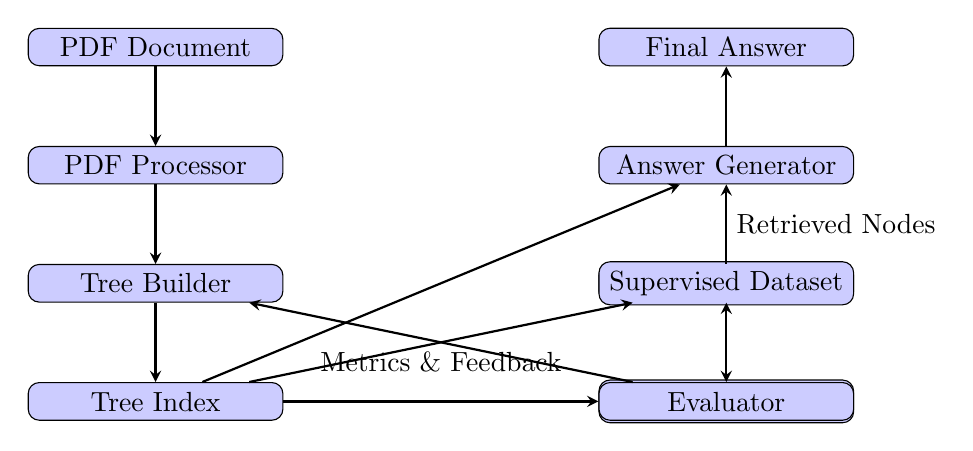
\begin{tikzpicture}[
    node distance=1.5cm,
    box/.style={rectangle, draw, fill=blue!20, text width=3cm, align=center, rounded corners},
    arrow/.style={->, >=stealth, thick}
]

% Nodes
\node[box] (pdf) {PDF Document};
\node[box, below of=pdf] (extract) {PDF Processor};
\node[box, below of=extract] (tree) {Tree Builder};
\node[box, below of=tree] (index) {Tree Index};

\node[box, right=4cm of index] (query) {User Query};
\node[box, above of=query] (search) {LLM Tree Searcher};
\node[box, above of=search] (gen) {Answer Generator};
\node[box, above of=gen] (answer) {Final Answer};

\node[box, right=4cm of tree] (sup) {Supervised Dataset};
\node[box, below of=sup] (eval) {Evaluator};

% Arrows
\draw[arrow] (pdf) -- (extract);
\draw[arrow] (extract) -- (tree);
\draw[arrow] (tree) -- (index);

\draw[arrow] (query) -- (search);
\draw[arrow] (index) -- (search);
\draw[arrow] (search) -- node[right] {Retrieved Nodes} (gen);
\draw[arrow] (index) -- (gen);
\draw[arrow] (gen) -- (answer);

\draw[arrow] (sup) -- (eval);
\draw[arrow] (index) -- (eval);
\draw[arrow] (eval) -- node[below] {Metrics \& Feedback} (tree);

\end{tikzpicture}
\caption{Vectorless RAG System Architecture}
\end{figure}

\subsection{Key Classes}

\subsubsection{TreeNode Class}

\begin{lstlisting}[language=Python, caption=TreeNode Implementation]
@dataclass
class TreeNode:
    """Node in document tree"""
    node_id: str
    title: str
    page_start: int
    page_end: int
    level: int
    summary: Optional[str] = None
    content: Optional[str] = None
    children: List['TreeNode'] = None
    
    def __post_init__(self):
        if self.children is None:
            self.children = []
    
    def to_dict(self) -> Dict:
        """Serialize to JSON"""
        return {
            'node_id': self.node_id,
            'title': self.title,
            'page_start': self.page_start,
            'page_end': self.page_end,
            'level': self.level,
            'summary': self.summary,
            'content': self.content,
            'children': [
                child.to_dict()
                for child in self.children
            ]
        }
\end{lstlisting}

\subsubsection{VectorlessRAG Class}

\begin{lstlisting}[language=Python, caption=Main RAG Class]
class VectorlessRAG:
    """Main RAG system"""
    
    def __init__(self, openai_api_key: str):
        self.client = OpenAI(api_key=openai_api_key)
        self.pdf_processor = PDFProcessor()
        self.tree_builder = TreeBuilder(self.client)
        self.searcher = LLMTreeSearcher(self.client)
        self.tree = None
    
    def index_document(
        self,
        pdf_path: str,
        cache_path: Optional[str] = None
    ) -> TreeNode:
        """Index PDF and build tree"""
        # Extract pages
        pages = self.pdf_processor.extract_pages(
            pdf_path
        )
        
        # Build tree
        self.tree = self.tree_builder.build_tree(
            pages
        )
        
        # Cache if requested
        if cache_path:
            self._save_tree(cache_path)
        
        return self.tree
    
    def query(
        self,
        question: str,
        max_nodes: int = 5
    ) -> Dict[str, Any]:
        """Query indexed document"""
        # Search tree
        node_ids = self.searcher.search(
            question, self.tree, max_nodes
        )
        
        # Retrieve nodes
        nodes = self._retrieve_nodes(node_ids)
        
        # Generate answer
        answer = self._generate_answer(
            question, nodes
        )
        
        return {
            'answer': answer,
            'sources': [
                {
                    'title': n.title,
                    'pages': f"{n.page_start}-{n.page_end}"
                }
                for n in nodes
            ],
            'node_ids': node_ids
        }
\end{lstlisting}

\subsection{Configuration}

\subsubsection{Environment Variables}

\begin{lstlisting}[language=bash, caption=.env File]
# OpenAI API Key
OPENAI_API_KEY=sk-your-key-here

# Model selection
LLM_MODEL=gpt-4o-mini

# Tree building parameters
MAX_PAGES_PER_NODE=10
TOC_CHECK_PAGES=20
GENERATE_SUMMARIES=true

# Retrieval parameters
MAX_RETRIEVED_NODES=5
\end{lstlisting}

% ============================================================================
\section{Usage Examples}
% ============================================================================

\subsection{Basic Usage}

\subsubsection{Complete Example}

\begin{lstlisting}[language=Python, caption=Basic Usage Example]
from vectorless_rag import VectorlessRAG
import os

# Initialize system
rag = VectorlessRAG(
    openai_api_key=os.getenv("OPENAI_API_KEY")
)

# Index a document
tree = rag.index_document(
    pdf_path="research_paper.pdf",
    cache_path="research_paper_tree.json"
)

# Print tree structure
rag.print_tree()

# Query the document
result = rag.query(
    "What methodology was used?",
    max_nodes=3
)

print("Answer:", result['answer'])
print("\nSources:")
for source in result['sources']:
    print(f"  - {source['title']} (pp. {source['pages']})")
\end{lstlisting}

\subsection{Supervised Evaluation}

\begin{lstlisting}[language=Python, caption=Evaluation Example]
from supervised_rag import (
    SupervisedRAGEvaluator,
    SupervisedQAPair
)

# Create evaluator
evaluator = SupervisedRAGEvaluator(
    openai_client=rag.client
)

# Add QA pairs
evaluator.add_qa_pair(
    question="What was the sample size?",
    ground_truth_answer="The study used 500 participants",
    relevant_node_ids=["node_0005"],
    context_needed="Methodology section",
    difficulty="easy",
    category="methods"
)

# Save for reuse
evaluator.save_qa_pairs("qa_dataset.json")

# Run evaluation
results = evaluator.evaluate_rag_system(
    rag_system=rag,
    verbose=True
)

# View metrics
print(results['aggregate_metrics']['summary'])
\end{lstlisting}

\end{document}
